\NewChapter{Shoot the Moon}

\quote{知己知彼,胜乃不怠;知天知地,胜乃不穷。}{孙武}

《Shoot the Moon》是一款本地双人对战游戏。游戏目标是控制自己的砖块移动,尽可能把在游戏场景内飞来飞去的小球反弹至月球,游戏会在有任意一方的砖块全部摧毁时结束,击中月球次数高的玩家获胜。\textbf{游戏Innovation得分排名 181 / 490。}

游戏创作于2020年11月,为Game Off 2020参赛作品,大赛主题为“MOONSHOT”,使用Godot游戏引擎单人参赛。游戏灵感源自打砖块,如果打砖块中接球的板子就是砖块本身,砖块的数量就是玩家的生命,会发生什么?为了控制击球方向,玩家必须牺牲生命、加速游戏进程,如何把握时机防止成为落水狗?如何利用中间的月球调整自己的阵型不让对方得分?快来尝试吧!!

\begin{figure}[H]
\centering  %图片全局居中
\subfigure[没有美术是这样的]{
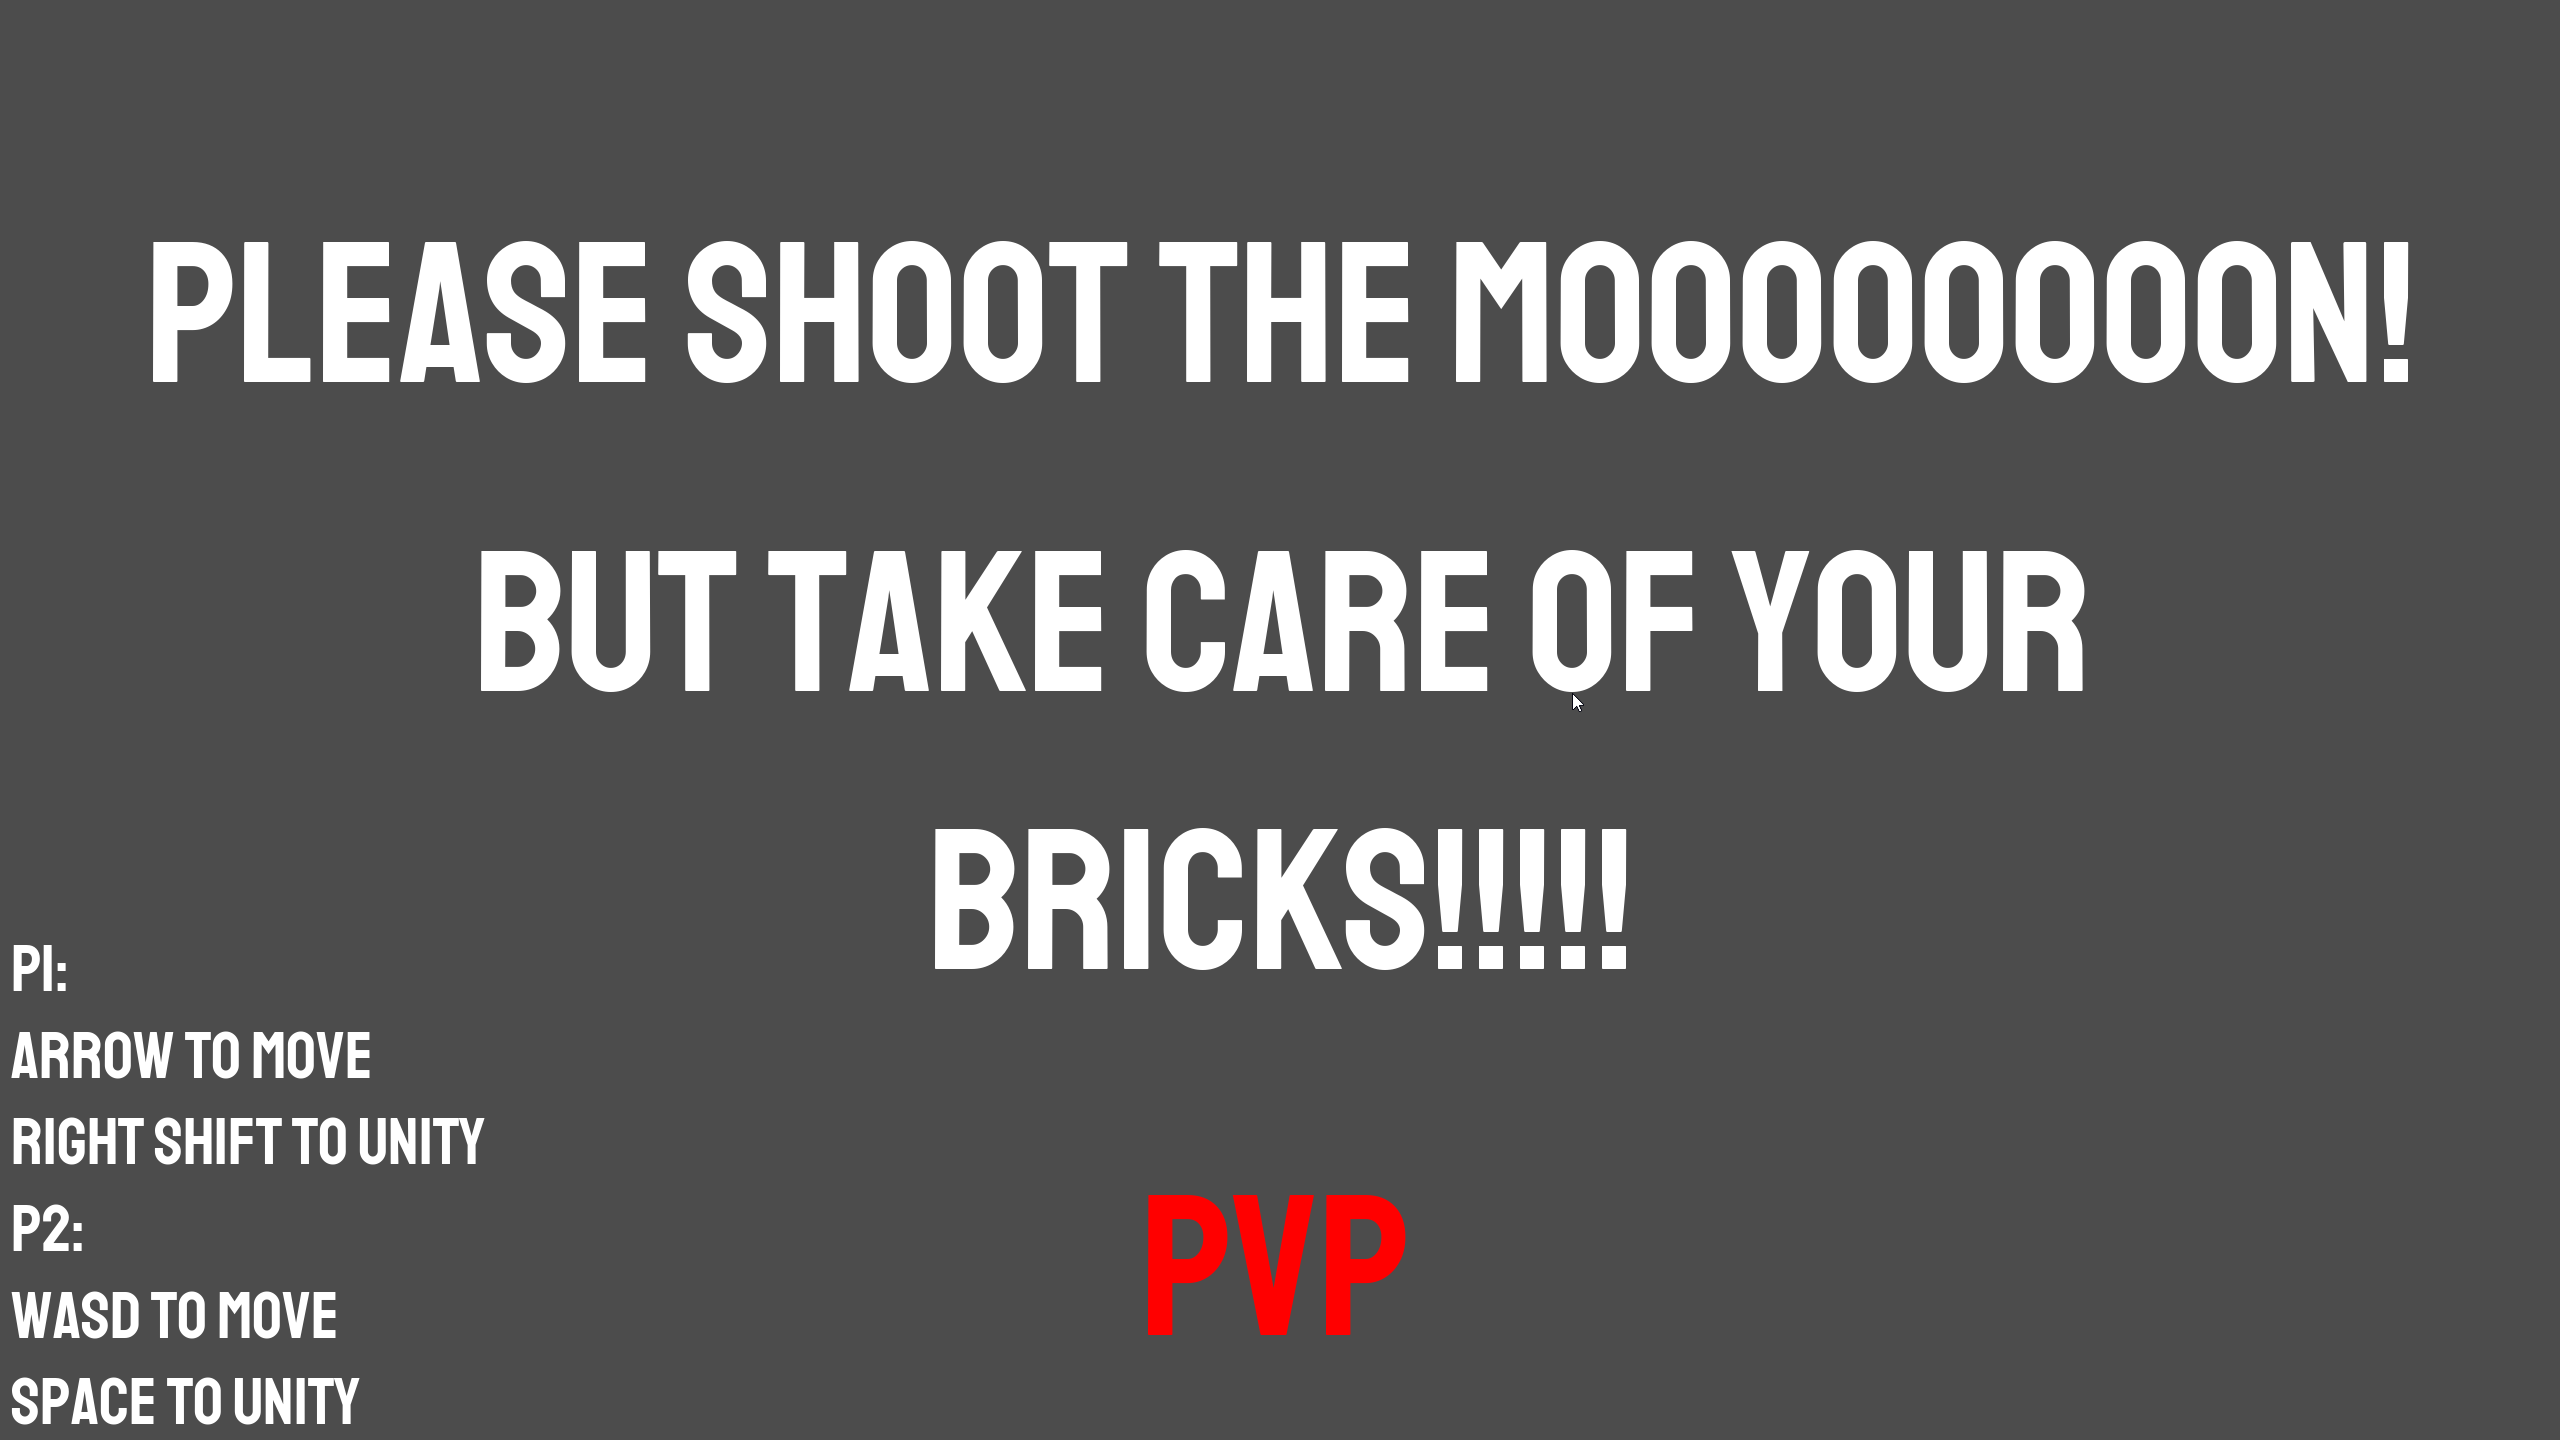
\includegraphics[width=0.45\textwidth]{Images/Shoot the Moon/Poster.png}}
\subfigure[游戏画面1]{
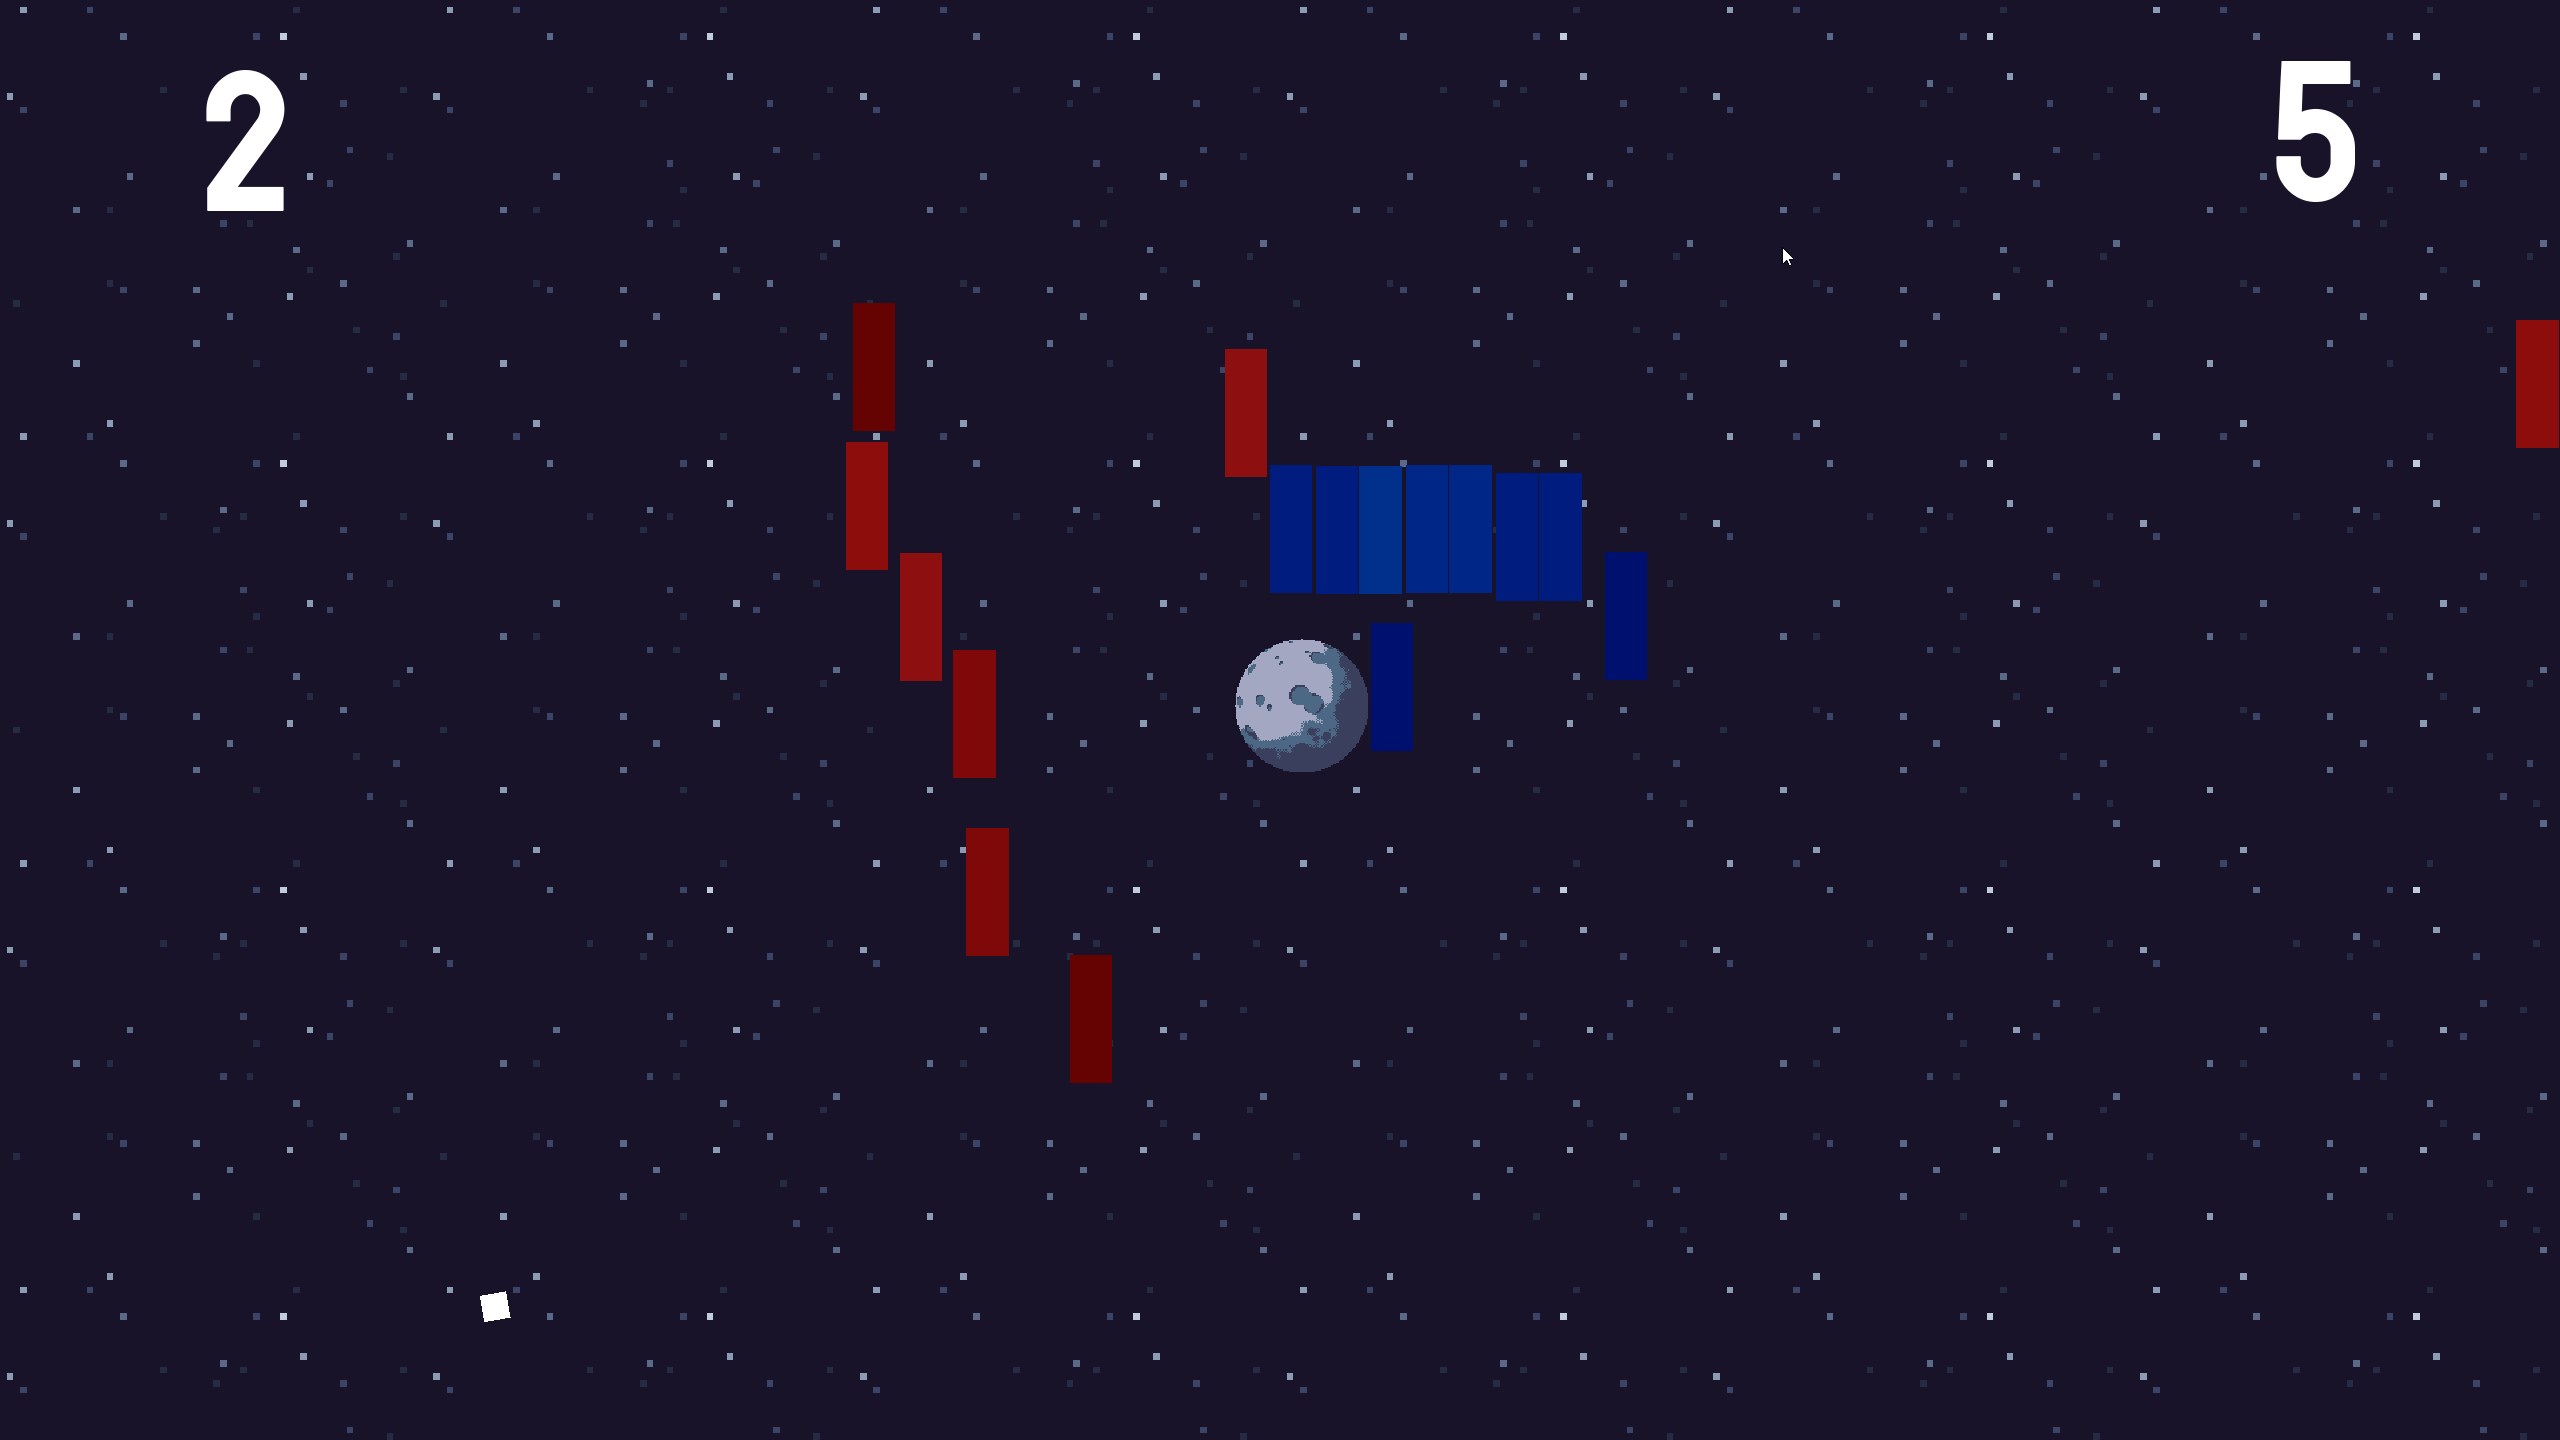
\includegraphics[width=0.45\textwidth]{Images/Shoot the Moon/STM1.png}}

\subfigure[游戏画面2]{
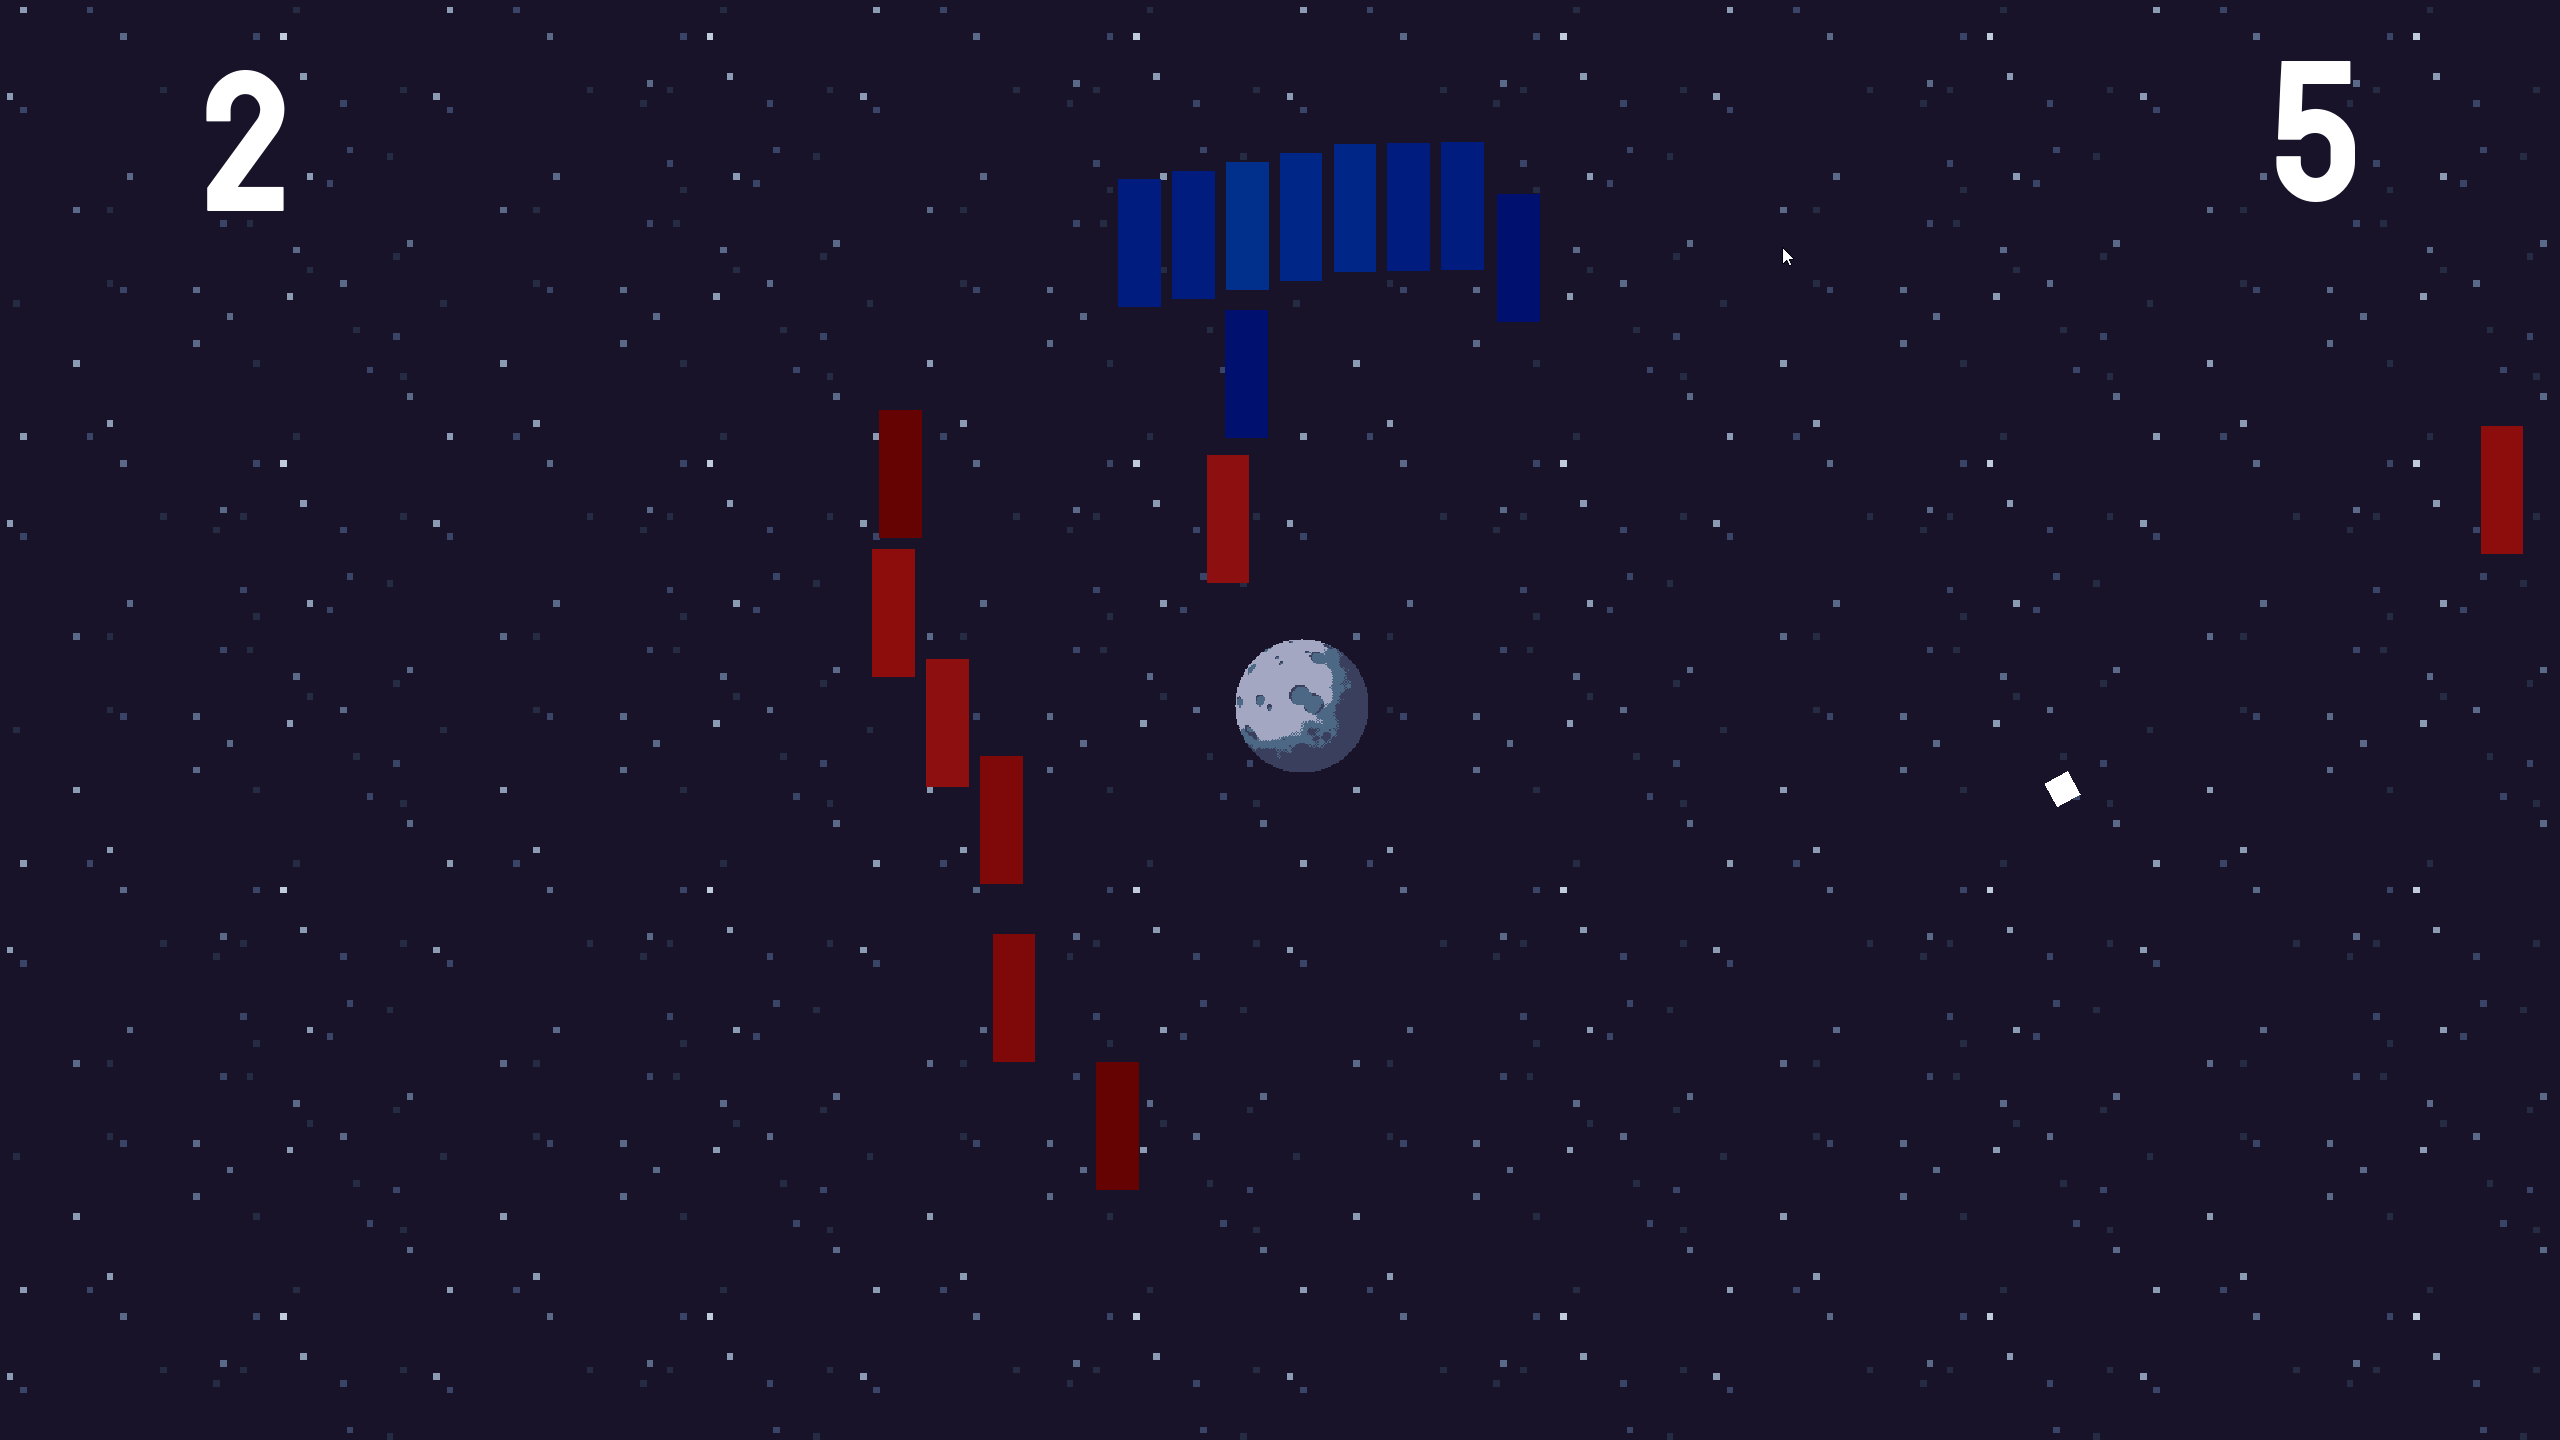
\includegraphics[width=0.45\textwidth]{Images/Shoot the Moon/STM2.png}}
\subfigure[蓝色方胜利]{
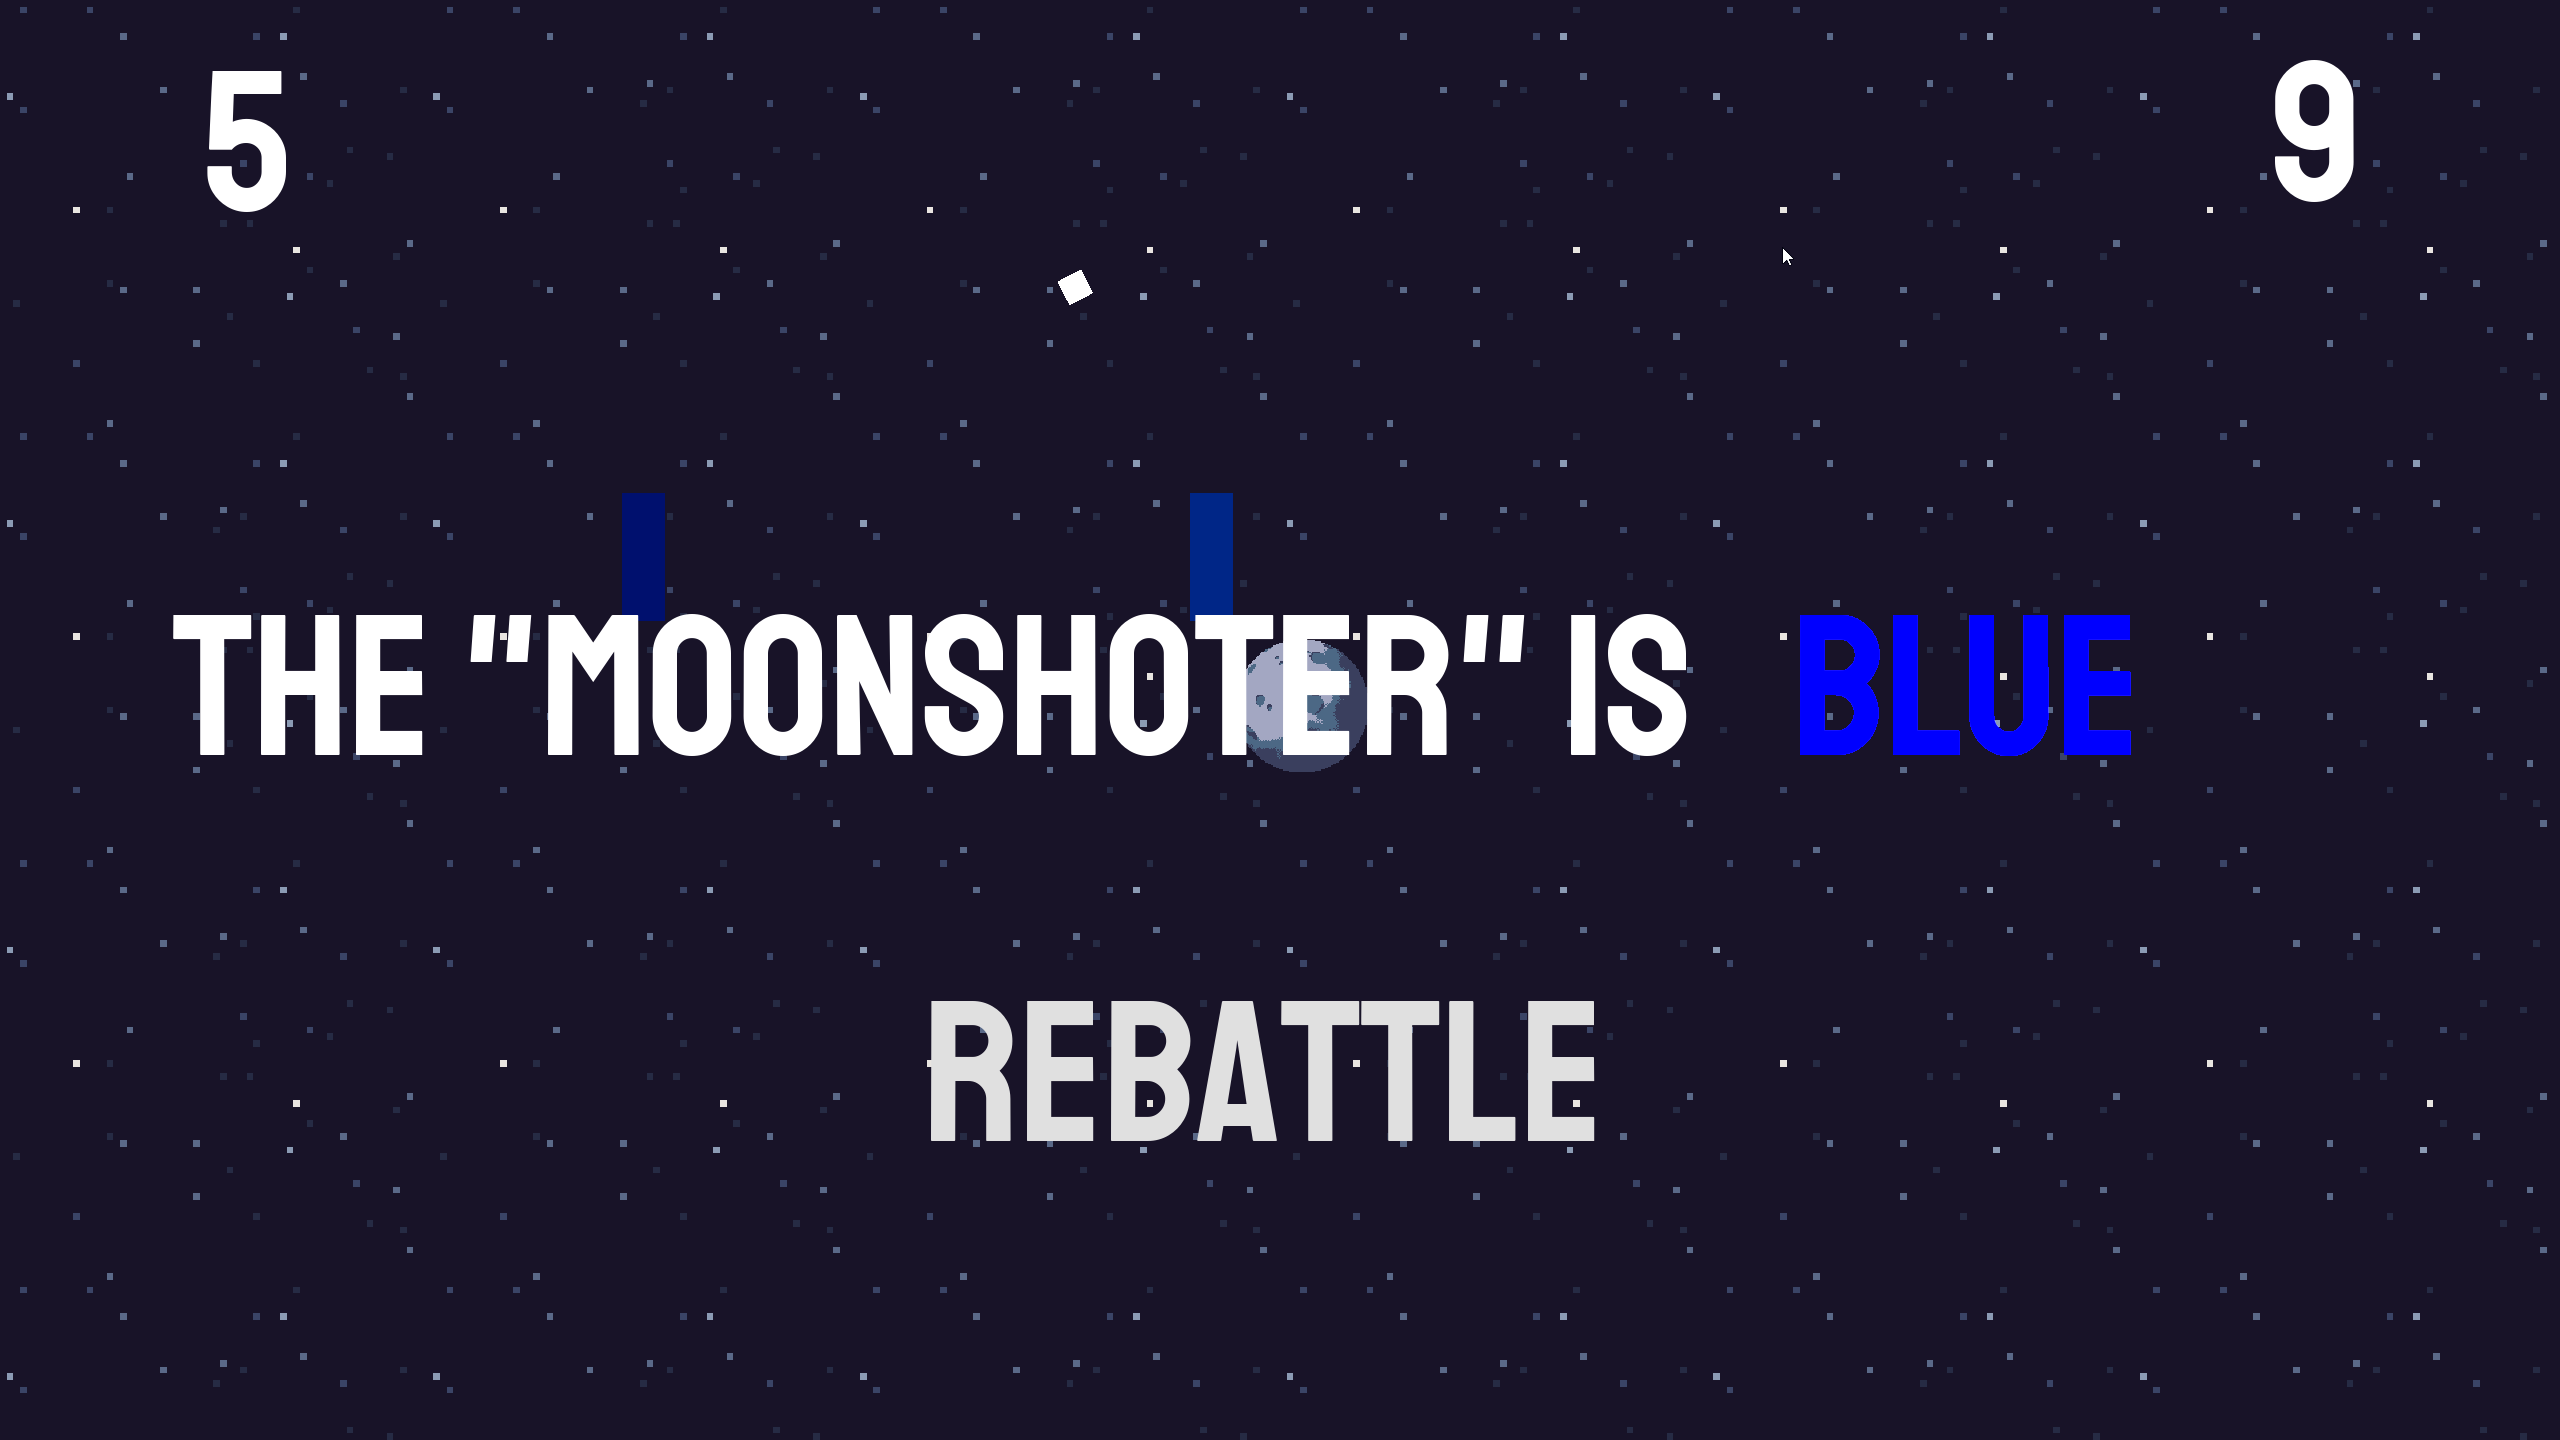
\includegraphics[width=0.45\textwidth]{Images/Shoot the Moon/STMWin.png}}
\caption{Shoot the Moon\ 游戏画面}
\end{figure}


\begin{itemize}
    \item \textbf{试玩视频:} \href{https://www.bilibili.com/video/BV1U24y137PN/?vd_source=ead0ac501dfae814e19fd7d9f376d92d}{Bilibili视频}
    \item \textbf{参赛页面:} \href{https://itch.io/jam/game-off-2020/rate/839864}{Game Off 2020}
    \item \textbf{Demo下载:} \href{https://scyq.itch.io/shoot-the-moon}{itch.io页面}
\end{itemize}
